\documentclass[11pt]{article}
\begin{document}
\title{5.0 Anhang}
\maketitle
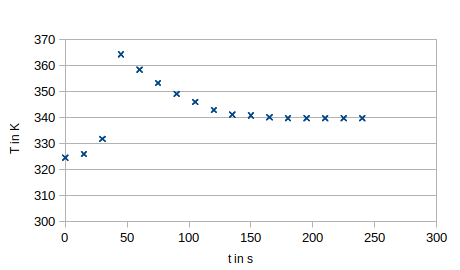
\includegraphics[scale=1]{/home/janosch/Schreibtisch/UHB/SEM2/PHY-B/Praktikum/[1]T5/Wachs.png}
\begin{flushleft}
\small Abb.1: Auftragung der in Tab. 1 aufgeführten Wertepaare.
\end{flushleft}
\includegraphics[scale=1]{/home/janosch/Schreibtisch/UHB/SEM2/PHY-B/Praktikum/[1]T5/Messingkörper.png}
\begin{flushleft}
\small Abb.2: Auftragung der in Tab.2 aufgeführten Werte von ln(T) über die Zeit. Die Blaue Wertereihe stellt die Werte des Kleinen Messingkörpers dar, Während die Orange Wertereihe die Messdaten des Großen Messingkörpers darstellt.\\
$R^2_{\text{Klein}}=0,999872577306472\approx 0,99$ $R^2_{\text{Groß}}=0,999005346732795\approx 0,99$
\end{flushleft}

\end{document}

